\chapter{Análisis de duplicaciones génicas en una selección de cepas bacterianas}
\label{chapter: analisis}

%% reorganizado
Con el fin de complementar la caracterización de duplicidades en cepas de \textit{E. coli} y diferentes especies de estafilococos y enterococos descritas anteriormente \cite{bernabeu_gene_2019, sanchez-herrero_gene_2020} y como ejemplo de uso de las herramientas desarrolladas durante este TFM descritas en el capítulo \ref{chapter: desarrollo} se ha hecho un análisis de la duplicación génica en cepas bacterianas del grupo ESKAPE. Se han utilizado las especies del grupo no incluidas en estos trabajos (\textbf{\textit{Klebsiella pneumoniae, Acinetobacter baumannii, Pseudomonas aeruginosa, Enterobacter} spp.}.

Este grupo de bacterias se caracteriza por ser especialmente patógenas al presentar resistencia a los antibióticos conocidos para el tratamiento de las enfermedades derivadas de ellas \cite{pendleton_clinical_2013, chavez-jacobo_batalla_2020}. Son bacterias Gram-negativas de marcado comportamiento oportunista que colonizan las vías respiratorias y digestivas de individuos inmunodeprimidos provocando infecciones y neumonías graves. Al ser muy resistentes a los antibióticos conocidos su tratamiento puede complicarse llegando a la muerte del paciente \cite{toro_klebsiella_2010, farinas_infecciones_2013, todar_pseudomonas_nodate, dworkin_genus_2006}. 

\section{Selección de cepas}

Para realizar la selección de cepas a analizar, se ha procedido a realizar una búsqueda en la base de datos de genomas del NCBI \cite{noauthor_home_nodate} para cada una de las especies a estudio. Se han filtrado los resultados para obtener genomas completos y patógenas para el ser humano, los resultados obtenidos se ordenaron por fecha de actualización y se eligieron las cuatro cepas más actuales de cada especie (figura \ref{fig:busqueda_ncbi}). En la tabla \ref{table:cepas} se muestran las cepas seleccionadas.

\begin{figure}
	\centering
	\captionsetup{width=\linewidth} 
	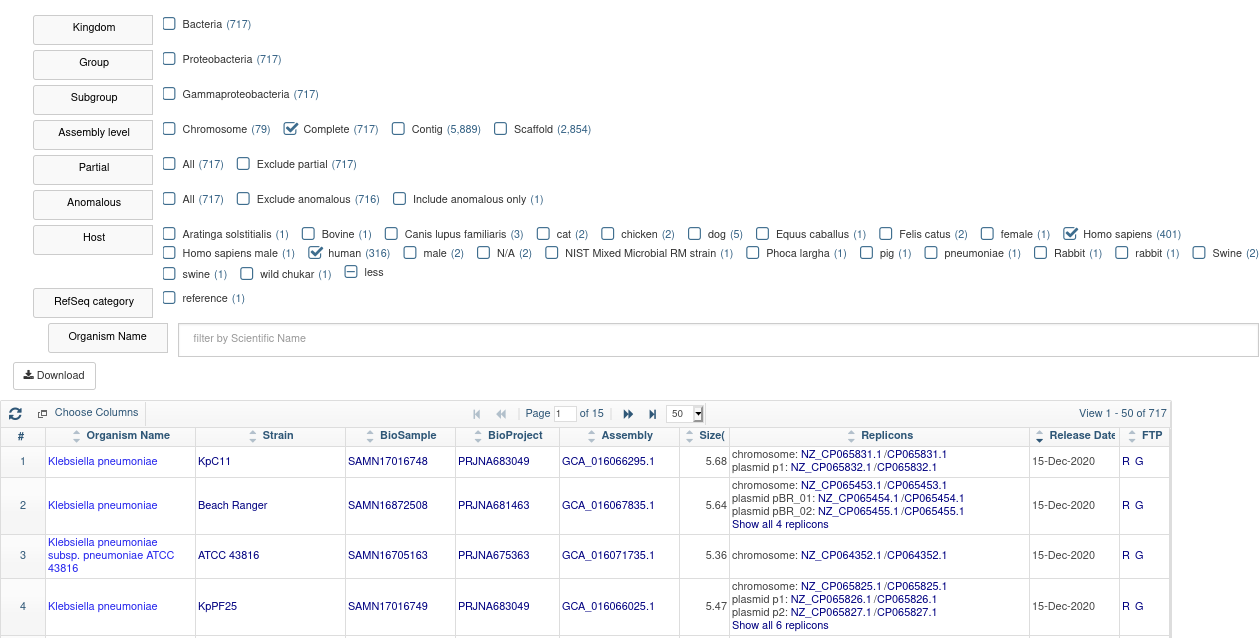
\includegraphics[width=\linewidth]{figs/busqueda_ncbi.png}
	\caption[Filtro de resultados de NCBI]{Resultados obtenidos en NCBI al hacer una búsqueda de la cepa de interés y aplicar los filtros deseados. Los resultados se han ordenado por fecha de actualizaciónn para poder seleccionar las cepas con los datos más actualizados.}
	\label{fig:busqueda_ncbi}
\end{figure}

\begin{table}
	\centering
	\captionsetup{width=0.5\linewidth}
	\begin{tabular}{ l || c }
		\hline
		Especie & Cepa\\
		\hline
		\hline
		\multirow{4}{*}{\textit{Klebsiella pneumoniae}} & KpC11 \\
		%\hline
		& ATCC 43816 \\
		%\hline
		& Beach Ranger \\
		%\hline
		& KpPF25 \\
		\hline
		\multirow{4}{*}{\textit{Acinetobacter baumannii}} & ATCC 17961 \\
		%\hline
		& TP3 \\
		%\hline
		& TP2 \\
		%\hline
		& FDAARGOS\_1036 \\
		\hline
		\multirow{4}{*}{\textit{Pseudomonas aeruginosa}} & DL201330 \\
		%\hline
		& TJ2014-049 \\
		%\hline
		& TJ2019-017 \\
		%\hline
		& TJ2019-022 \\
		\hline
		\multirow{4}{*}{\textit{Enterobacter cloacae}} & STN0717-73  \\
		& STN0717-60  \\
		& RHBSTW-00399  \\
		& RHBSTW-00490  \\
		\hline
	\end{tabular}
	\caption{Cepas seleccionadas para llevar a cabo la búsqueda de duplicidades y ejemplo de uso de la herramienta.}
	\label{table:cepas}
\end{table}


\newpage
\section{Búsqueda y representación de duplicidades}

A continuación se muestra como ejemplo de uso de las herramientas desarrolladas en la búsqueda, anotación y representación de duplicidades génicas de la cepa Beach Ranger de \textit{Klebsiella pneumoniae}. El motivo de la elección de esta cepa como muestra de ejemplo es meramente didáctico. Es un grupo de bacterias con varios plásmidos de diferentes tamaños y muestra duplicidades tanto en las hebras positivas como negativas. Estas características se prestan a generar unas gráficas visualmente atractivas y completas para explicar cada uno de los elementos que nos encontramos.

\paragraph{\textbf{- Datos: }} Los archivos de anotación completos se pueden descargar directamente del servidor de búsqueda del NCBI, accediendo a la carpeta ftp del servidor (figura \ref{fig:ncbi_beach}) desde el link que se ofrece en la columna correspondiente. Si se desea el genoma del cromosoma o un plásmido en concreto, se puede acceder a ellos directamente desde los enlaces de la tabla de resultados de búsqueda.

\begin{figure}[h]
	\centering
	\captionsetup{width=0.6\linewidth} 
	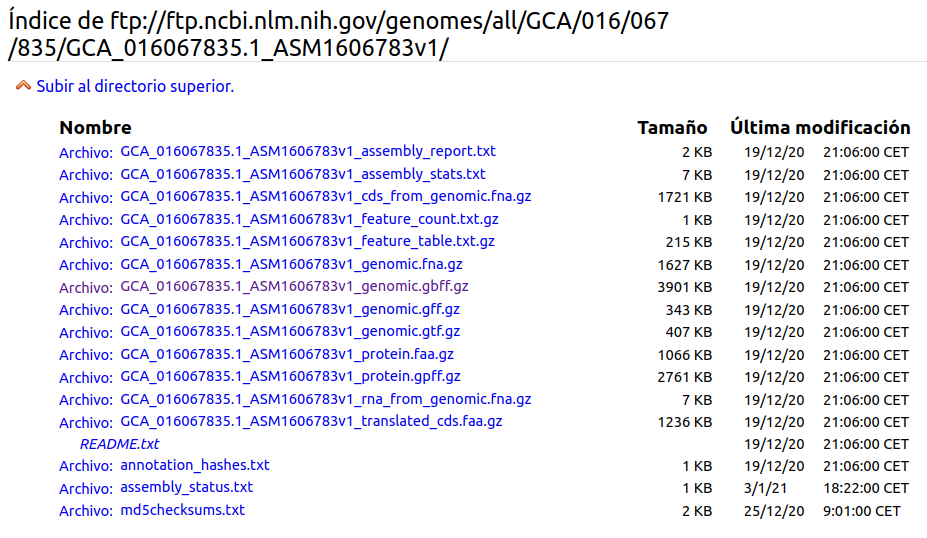
\includegraphics[width=0.6\linewidth]{figs/ncbi_beach.png}
	\caption[Carpeta ftp de NCBI]{Contenido de archivos de la carpeta correspondiente a la cepa Beach Ranger del servidor ftp de NCBI}
	\label{fig:ncbi_beach}
\end{figure}

Hemos seleccionado la anotación en formato \textit{GenBank} (extensión gbff) ya que nos permite utilizar un único documento, favoreciendo la agilidad del proceso.

\paragraph{\textbf{- Búsqueda y anotación de duplicados: }} Siguiendo las indicaciones dadas en el capítulo anterior. Invocamos desde la terminal el módulo dup\_annot.py y aportamos la información conveniente. Dejamos los valores de los parámetros que se dan por defecto y generamos los resultados (figura \ref{fig:ex_beach}).

\begin{figure}[h]
	\centering
	\captionsetup{width=0.7\linewidth} 
	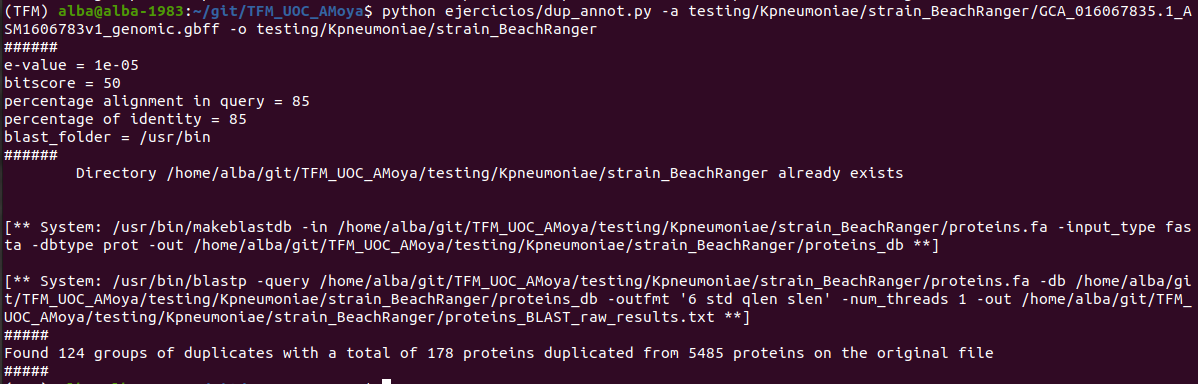
\includegraphics[width=0.7\linewidth]{figs/ex_beach.png}
	\caption[Ejemplo de uso en la cepa Beach Ranger]{Resultados obtenidos en la terminal al invocar dup\_annot.py con los datos para la cepa Beach Ranger.}
	\label{fig:ex_beach}
\end{figure}

\newpage
\paragraph{\textbf{- Resultados obtenidos: }} La figura \ref{fig:beach_result} muestra un fragmento de la tabla de anotación para esas 178 proteínas duplicadas en la cepa Beach Ranger.

\begin{figure}[h]
	\centering
	\captionsetup{width=\linewidth} 
	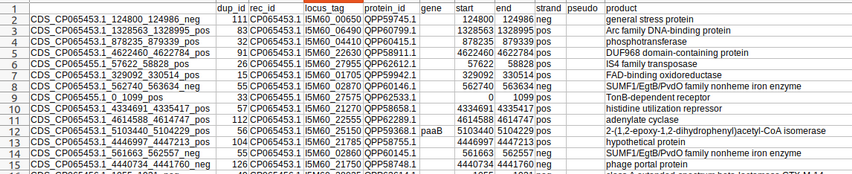
\includegraphics[width=\linewidth]{figs/beach_result.png}
	\caption[Tabla de anotación del genoma duplicado de la cepa Beach Ranger]{Tabla de anotación de las proteínas duplicadas generada tras el tratamiento de los datos de la cepa Beach Rangercon input\_parser.py}
	\label{fig:beach_result}
\end{figure}

En el apéndice \ref{apB} se puede encontrar los resultados obtenidos para la totalidad de las cepas estudiadas.

\paragraph{\textbf{- Representación gráfica: }} Finamente, utilizando los comandos de R procedemos a generar la gráfica que nos mostrará la distribución de las proteínas duplicadas. 

Le indicamos al programa cuáles son los datos que debe utilizar con las siguientes instrucciones: 

\vspace{5mm}
\begin{lstlisting}[language=R]
## strain BeachRanger
seq_lengths_BeachRanger <- read.csv(paste0(data_folder, "Kpneumoniae/strain_BeachRanger/length.csv"),
                                  header=FALSE, row.names=1)
bed_info_file_BeachRanger <- read.table(paste0(data_folder, "Kpneumoniae/strain_BeachRanger/dup_annot.csv"), sep=",",
                                      header=TRUE)
bed_info_file_BeachRanger <- bed_info_file_BeachRanger[,c("dup_id", "rec_id", "start", "end", "locus_tag", "product", "strand")]
\end{lstlisting}
\vspace{5mm}

Se debe considerar que el valor por defecto para los pseudogenes en dup\_annot es no tenerlos en cuenta a la hora de generar la tabla final, pero sí que se incluyeron en los grupos de duplicados correspondiente. Esto puede resultar en que nos queden grupos de duplicados con una única proteína, lo que nos generará problemas a la hora de intentar graficar los resultados. Para evitar esto, eliminamos esas proteínas huérfanas con el siguiente comando:

\vspace{5mm}
\begin{lstlisting}[language=R]
# # keep only real duplicated groups
bed_info_file_BeachRanger <- bed_info_file_BeachRanger %>% group_by(dup_id) %>% filter(n() >1)
# 
\end{lstlisting}
\vspace{5mm}

Finalmente, creamos nuestro BioCircos (figura \ref{fig:biobeach}):

\vspace{5mm}
\begin{lstlisting}[language=R]
create_BioCircos(seq_lengths = seq_lengths_BeachRanger,
                 bed_info_file = bed_info_file_BeachRanger)
\end{lstlisting}
\vspace{5mm}

\begin{figure}[h]
	\centering
	\captionsetup{width=\linewidth} 
	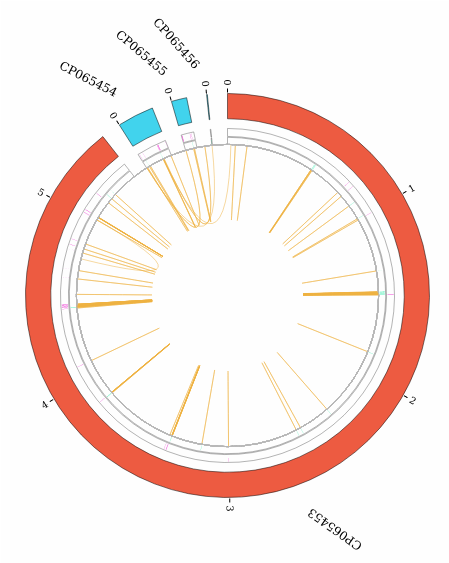
\includegraphics[width=\linewidth]{figs/biocircos_BeachRanger.png}
	\caption[Gráfica biocircos para la cepa Beach Ranger de \textit{K. pneumoniae}]{Representación gráfica con BioCircos de los genes duplicados en el genoma de la cepa Beach Ranger de \textit{K. pneumoniae}. El cromosoma de la bacteria (rojo) y sus plásmidos (azul) se representan en un mapa circular que muestra la localización de cada gen duplicado. Las siguientes dos capas muestran los genes en la hebra positiva (rosa) y negativa (turquesa). Las líneas naranja interiores señalan las conexiones entre proteínas pertenecientes al mismo grupo de duplicados. Escala de tamaño en Mb}
	\label{fig:biobeach}
\end{figure}

En el apéndice \ref{apB} se adjunta los cuatro gráficos correspondientes a cada cepa de \textit{K pneumoniae} seleccionada con objetivo comparativo. También se aporta el enlace a la carpeta github correspondiente donde encontrar todas las gráficas de las cepas analizadas y los archivos generados tras su análisis.